%%%%%%%%%%%%%%%%%%%%%%%%%%%%%%%%%%%%%%%%%%%%%%%
%
% Template per Elaborato di Laurea
% DISI - Dipartimento di Ingegneria e Scienza dell’Informazione
%
% update 2015-09-10
%
% Per la generazione corretta del 
% pdflatex nome_file.tex
% bibtex nome_file.aux
% pdflatex nome_file.tex
% pdflatex nome_file.tex
%
%%%%%%%%%%%%%%%%%%%%%%%%%%%%%%%%%%%%%%%%%%%%%%%

% formato FRONTE RETRO
\documentclass[epsfig,a4paper,11pt,titlepage,twoside,openany]{book}
\usepackage{epsfig}
\usepackage{plain}
\usepackage{setspace}
\usepackage[paperheight=29.7cm,paperwidth=21cm,outer=1.5cm,inner=2.5cm,top=2cm,bottom=2cm]{geometry} % per definizione layout
\usepackage{titlesec} % per formato custom dei titoli dei capitoli

%%%%%%%%%%%%%%
% supporto lettere accentate
%
%\usepackage[latin1]{inputenc} % per Windows;
\usepackage[utf8x]{inputenc} % per Linux (richiede il pacchetto unicode);
\usepackage[T1]{fontenc}
%\usepackage[applemac]{inputenc} % per Mac.

\singlespacing

\usepackage[italian]{babel}

% aggiunti da Valerio Asaro
\usepackage[hidelinks]{hyperref}

% per i .png
\usepackage{graphicx}

% per le tabelle
\usepackage{array}

% per formule matematiche
\usepackage{amsmath}

% per fare stare i grafici al loro posto
\usepackage{float}

% per snippets di codice
\usepackage{xcolor}
\usepackage{listings}

\definecolor{codegreen}{rgb}{0.0,0.45,0.2}
\definecolor{codegray}{rgb}{0.45,0.45,0.45}
\definecolor{codepurple}{rgb}{0.55,0.2,0.65}
\definecolor{codeblue}{rgb}{0.1,0.2,0.7}

\lstset{
	language=Python,
	basicstyle=\ttfamily\small,
	keywordstyle=\color{codeblue}\bfseries,
	commentstyle=\color{codegreen}\itshape,
	stringstyle=\color{codepurple},
	identifierstyle=\color{black},
	numbers=left,
	numberstyle=\tiny\color{codegray},
	stepnumber=1,
	frame=single,
	breaklines=true,
	captionpos=b,
	showstringspaces=false,
	keepspaces=true,
	tabsize=4
}

\begin{document}

  % nessuna numerazione
  \pagenumbering{gobble} 
  \pagestyle{plain}

\thispagestyle{empty}

\begin{center}
  \begin{figure}[h!]
    \centerline{\psfig{file=marchio_unitrento_colore_it_202002.eps,width=0.6\textwidth}}
  \end{figure}

  \vspace{2 cm} 

  \LARGE{Dipartimento di Ingegneria e Scienza dell’Informazione\\}

  \vspace{1 cm} 
  \Large{Corso di Laurea in\\
    ...
    Informatica
    %Ingegneria dell'Informazione e delle Comunicazioni
    %Ingegneria dell'Informazione e Organizzazione d'Impresa
    %Ingegneria Elettronica e delle Telecomunicazioni
  }

  \vspace{2 cm} 
  \Large\textsc{Elaborato finale\\} 
  \vspace{1 cm} 
  \Huge\textsc{Titolo\\}
  \Large{\it{Sottotitolo (alcune volte lungo - opzionale)}}


  \vspace{2 cm} 
  \begin{tabular*}{\textwidth}{ c @{\extracolsep{\fill}} c }
  \Large{Supervisore} & \Large{Laureando}\\
  \Large{......}& \Large{......}\\
  \end{tabular*}

  \vspace{2 cm} 

  \Large{Anno accademico 2026/2027}
  
\end{center}



  \clearpage
 
%%%%%%%%%%%%%%%%%%%%%%%%%%%%%%%%%%%%%%%%%%%%%%%%%%%%%%%%%%%%%%%%%%%%%%%%%%
%%%%%%%%%%%%%%%%%%%%%%%%%%%%%%%%%%%%%%%%%%%%%%%%%%%%%%%%%%%%%%%%%%%%%%%%%%
%% Nota
%%%%%%%%%%%%%%%%%%%%%%%%%%%%%%%%%%%%%%%%%%%%%%%%%%%%%%%%%%%%%%%%%%%%%%%%%%
%% Sezione Ringraziamenti opzionale
%%%%%%%%%%%%%%%%%%%%%%%%%%%%%%%%%%%%%%%%%%%%%%%%%%%%%%%%%%%%%%%%%%%%%%%%%%
%%%%%%%%%%%%%%%%%%%%%%%%%%%%%%%%%%%%%%%%%%%%%%%%%%%%%%%%%%%%%%%%%%%%%%%%%%
  \thispagestyle{empty}

\begin{center}
  {\bf \Huge Ringraziamenti}
\end{center}

\vspace{4cm}


\emph{
per il momento vorrei ringraziare i miei due gentilissimi correlatori per il loro immenso aiuto nella stesura di questo documento :D
}

  \clearpage
  \pagestyle{plain} % nessuna intestazione e pie pagina con numero al centro

  
  % inizio numerazione pagine in numeri arabi
  \mainmatter

%%%%%%%%%%%%%%%%%%%%%%%%%%%%%%%%%%%%%%%%%%%%%%%%%%%%%%%%%%%%%%%%%%%%%%%%%%
%%%%%%%%%%%%%%%%%%%%%%%%%%%%%%%%%%%%%%%%%%%%%%%%%%%%%%%%%%%%%%%%%%%%%%%%%%
%% Nota
%%%%%%%%%%%%%%%%%%%%%%%%%%%%%%%%%%%%%%%%%%%%%%%%%%%%%%%%%%%%%%%%%%%%%%%%%%
%% Si ricorda che il numero massimo di facciate e' 30.
%% Nel conteggio delle facciate sono incluse 
%%   indice
%%   sommario
%%   capitoli
%% Dal conteggio delle facciate sono escluse
%%   frontespizio
%%   ringraziamenti
%%   allegati    
%%%%%%%%%%%%%%%%%%%%%%%%%%%%%%%%%%%%%%%%%%%%%%%%%%%%%%%%%%%%%%%%%%%%%%%%%%
%%%%%%%%%%%%%%%%%%%%%%%%%%%%%%%%%%%%%%%%%%%%%%%%%%%%%%%%%%%%%%%%%%%%%%%%%%

    % indice
    \tableofcontents
    \clearpage
    
    
          
    % gruppo per definizone di successione capitoli senza interruzione di pagina
    \begingroup
      % nessuna interruzione di pagina tra capitoli
      % ridefinizione dei comandi di clear page
      \renewcommand{\cleardoublepage}{} 
      \renewcommand{\clearpage}{} 
      % redefinizione del formato del titolo del capitolo
      % da formato
      %   Capitolo X
      %   Titolo capitolo
      % a formato
      %   X   Titolo capitolo
      
      \titleformat{\chapter}
        {\normalfont\Huge\bfseries}{\thechapter}{1em}{}
        
      \titlespacing*{\chapter}{0pt}{0.59in}{0.02in}
      \titlespacing*{\section}{0pt}{0.20in}{0.02in}
      \titlespacing*{\subsection}{0pt}{0.10in}{0.02in}
      
      % sommario
      \begin{flushright}
	\textit{«La Galassia infatti non è altro che un ammasso
		di innumerabili stelle disseminate a mucchi.»}
	\vspace{0.2cm}
	Galileo Galilei, \textit{Sidereus Nuncius}, 1610
\end{flushright}

\vspace{0.5cm}

\chapter*{Sommario} % senza numerazione
\label{sommario}

\addcontentsline{toc}{chapter}{Sommario} % da aggiungere comunque all'indice

  Sommario è un breve riassunto del lavoro svolto dove si descrive l'obiettivo, l'oggetto della tesi, le 
metodologie e le tecniche usate, i dati elaborati e la spiegazione delle conclusioni alle quali siete arrivati.  

Il sommario dell’elaborato consiste al massimo di 3 pagine e deve contenere le seguenti informazioni:
\begin{itemize}
  \item contesto e motivazioni 
  \item breve riassunto del problema affrontato
  \item tecniche utilizzate e/o sviluppate
  \item risultati raggiunti, sottolineando il contributo personale del laureando/a
\end{itemize}





      \endgroup
%%%%%%%%%%%%%%%%%%%%%%%%%%%%%%%%%%%%%%%%%%%%%%%%%%%%%%%%%%%%%%%%%%%%%%%%%%
%%%%%%%%%%%%%%%%%%%%%%%%%%%%%%%%%%%%%%%%%%%%%%%%%%%%%%%%%%%%%%%%%%%%%%%%%%
%% Nota
%%%%%%%%%%%%%%%%%%%%%%%%%%%%%%%%%%%%%%%%%%%%%%%%%%%%%%%%%%%%%%%%%%%%%%%%%%
%% Sommario e' un breve riassunto del lavoro svolto dove si descrive 
%% l’obiettivo, l’oggetto della tesi, le metodologie e 
%% le tecniche usate, i dati elaborati e la spiegazione delle conclusioni 
%% alle quali siete arrivati.
%% Il sommario dell’elaborato consiste al massimo di 3 pagine e deve contenere le seguenti informazioni: 
%%   contesto e motivazioni
%%   breve riassunto del problema affrontato
%%   tecniche utilizzate e/o sviluppate
%%   risultati raggiunti, sottolineando il contributo personale del laureando/a
%%%%%%%%%%%%%%%%%%%%%%%%%%%%%%%%%%%%%%%%%%%%%%%%%%%%%%%%%%%%%%%%%%%%%%%%%%
%%%%%%%%%%%%%%%%%%%%%%%%%%%%%%%%%%%%%%%%%%%%%%%%%%%%%%%%%%%%%%%%%%%%%%%%%%      
      
	\begingroup
      %%%%%%%%%%%%%%%%%%%%%%%%%%%%%%%%
      % lista dei capitoli
      %
      % \input oppure \include
      %
      \chapter{Introduzione}
\label{cha:introduzione}

\section{Gli ammassi stellari}
\label{sec:ammassi-stellari}

Gli ammassi stellari sono sistemi gravitazionalmente legati,
costituiti da un insieme di stelle che interagiscono attraverso
la gravità. La loro evoluzione dipende sia dalla dinamica interna
sia dall'ambiente gravitazionale in cui si muovono
\cite{binneytremaine2008}.

Nel corso del tempo, le interazioni gravitazionali e l'influenza
del campo galattico possono modificare la distribuzione delle
stelle e provocare una perdita progressiva di massa. Comprendere
questi processi richiede di studiare come le condizioni iniziali
del sistema e le caratteristiche della sua orbita ne influenzino
l'evoluzione dinamica \cite{computationalmethods2023}.

Le simulazioni numeriche a molti corpi, o simulazioni
\textit{N-body}, permettono di seguire il moto delle singole
particelle e di ricostruire l'evoluzione del sistema nel tempo.
Esse costituiscono quindi uno strumento per analizzare gli
effetti delle interazioni gravitazionali e del campo esterno
sulla struttura di un ammasso stellare.

\section{Galactic Tidal Stripping}
\label{sec:galactic-tidal-stripping}

Un ammasso stellare che orbita all'interno di una galassia
è soggetto al campo gravitazionale galattico. La differenza
di accelerazione gravitazionale tra le diverse regioni
dell'ammasso produce effetti mareali, che possono favorire
la perdita di stelle e modificare la struttura del sistema.
Questo processo è noto come \textit{Galactic Tidal Stripping}.

L'intensità degli effetti mareali dipende, tra gli altri
fattori, dalla posizione dell'ammasso rispetto al centro
galattico e dalle caratteristiche della sua orbita.
In particolare, orbite differenti possono esporre l'ammasso
a condizioni gravitazionali differenti, influenzandone
l'evoluzione e la perdita di massa
\cite{baumgardt2003}.

Lo studio di questo fenomeno richiede pertanto di considerare
contemporaneamente la dinamica interna dell'ammasso e il suo
moto nel potenziale gravitazionale esterno. La complessità
del problema rende utile l'impiego di simulazioni numeriche,
che permettono di esaminare l'evoluzione del sistema per
diverse condizioni iniziali.

\section{Obiettivo}
\label{sec:obiettivo}


      \newcommand{\totalMass}{M}                        % Massa totale
\newcommand{\starMass}{m}                         % Massa singola stella
\newcommand{\numberOfStars}{N}                    % Numero di stelle
\newcommand{\radialDistance}{r}                   % Distanza radiale
\newcommand{\clusterRadius}{A}                    % Parametro di scala di Plummer 
\newcommand{\densityRho}{\rho}                    % Densità di massa
\newcommand{\potentialPhi}{\Phi}                  % Potenziale gravitazionale
\newcommand{\gravitationalConstant}{G}            % Costante gravitazionale
\newcommand{\escapeVelocity}{v_{\mathrm{esc}}}    % Velocità di fuga
\newcommand{\velV}{v}                             % Velocità
\newcommand{\totalCineticEnergy}{K}            	  % Energia Cinetica Totale
\newcommand{\totalPotentialEnergy}{U}             % Energia Potenziale Totale
\newcommand{\virialRatio}{Q}                      % Viriale
\newcommand{\semiMajorAxis}{a}                    % Semiasse Maggiore
\newcommand{\orbitEccentricity}{e}                % Eccentricità
\newcommand{\galaxyMass}{M_{\mathrm{gal}}}        % Massa galattica
\newcommand{\galaxyRadius}{A_{\mathrm{gal}}}    % Parametro di scala di Plummer 
\newcommand{\galaxyParameter}{b_{\mathrm{gal}}}   % Parametro potenziale galattico
\newcommand{\galaxyDistance}{R}                   % Distanza centro galattico
\newcommand{\velocityRescalingFactor}{\lambda}    % Fattore di riscalo per velocità
\newcommand{\deltat}{\Delta t}

\chapter{Il modello fisico}
\label{cha:modello-fisico}

\section{Notazione}
\label{sec:notazione}
La Tabella~\ref{tab:notazione} riassume i principali simboli utilizzati
nel capitolo.
\begin{table}[htbp]
	\centering
	\caption{Notazione utilizzata nel capitolo.}
	\label{tab:notazione}
	\begin{tabular}{ll}
		\hline
		\textbf{Simbolo} & \textbf{Significato} \\
		\hline
		$\numberOfStars$ & Numero di stelle dell'ammasso \\
		$\starMass$ & Massa di una singola stella \\
		$\totalMass$ & Massa totale dell'ammasso \\
		$\radialDistance$ & Distanza dal centro dell'ammasso \\
		$\clusterRadius$ & Parametro di scala del modello di Plummer \\
		$\mathbf{x}_i$ & Vettore posizione della stella $i$ \\
		$\mathbf{v}_i$ & Vettore velocità della stella $i$ \\
		$\gravitationalConstant$ & Costante gravitazionale \\
		$\densityRho(r)$ & Densità volumetrica di massa dell'ammasso \\
		$\potentialPhi(r)$ & Potenziale gravitazionale dell'ammasso \\
		$\galaxyMass$ & Massa del modello galattico \\
		$\galaxyRadius$ & Parametro di scala del modello di Plummer galattico \\
		$\galaxyParameter$ & Parametro di scala del potenziale galattico \\
		$\galaxyDistance$ & Distanza dal centro galattico \\
		$\semiMajorAxis$ & Semiasse maggiore dell'orbita dell'ammasso \\
		$\orbitEccentricity$ & Eccentricità dell'orbita dell'ammasso \\
		$\deltat$ & Passo temporale \\
		\hline
	\end{tabular}
\end{table}

\section{Generazione dell'ammasso stellare}
\label{sec:generazione-ammasso}
Per descrivere la distribuzione iniziale di un ammasso
stellare, si adotta il modello di Plummer,
che permette di definire la distribuzione delle posizioni
e delle velocità delle stelle nel contesto galattico.\cite{plummer1911}

\subsection{Il modello di Plummer}
\label{subsec:plummer}
Il modello di Plummer descrive un sistema
sferico autogravitante attraverso la sua distribuzione di massa.
È caratterizzato dalla massa totale $\totalMass$ e dal parametro
di scala $\clusterRadius$, che determina l'estensione della
distribuzione.\\
La densità volumetrica di massa in funzione della distanza
radiale $\radialDistance$ dal centro è \cite{plummer1911}:
\begin{equation}
	\densityRho(\radialDistance) =
	\frac{3\totalMass}{4\pi \clusterRadius^3}
	\left(1+\frac{\radialDistance^2}{\clusterRadius^2}\right)^{-5/2}
	\label{eq:plummer-density}
\end{equation}
Il potenziale gravitazionale associato alla distribuzione di
massa descritta dall'equazione~\eqref{eq:plummer-density}
si ottiene risolvendo l'equazione di Poisson
\cite{binneytremaine2008}:
\begin{equation}
	\potentialPhi(\radialDistance) =
	-\frac{\gravitationalConstant\totalMass}
	{\sqrt{\radialDistance^2+\clusterRadius^2}}
	\label{eq:plummer-potential}
\end{equation}

\subsection{Distribuzione delle posizioni}
\label{subsec:posizioni-iniziali}
Le posizioni iniziali delle stelle vengono estratte in modo da riprodurre la distribuzione spaziale descritta dal modello di Plummer. Integrando la densità definita nell'equazione~\eqref{eq:plummer-density} entro il raggio $\radialDistance$, si ottiene la frazione di massa racchiusa:
\begin{equation}
	\frac{M(\radialDistance)}{\totalMass}
	=
	\frac{\radialDistance^3}{(\radialDistance^2+\clusterRadius^2)^{3/2}}
	\label{eq:plummer-enclosed-mass}
\end{equation}
Questa quantità rappresenta la probabilità cumulativa di trovare una stella entro il raggio $\radialDistance$. Estraendo un numero casuale uniforme $u$ nell'intervallo $(0,1)$ e uguagliandolo a tale probabilità, si ricava il raggio iniziale di ciascuna stella:
\begin{equation}
	\radialDistance =
	\frac{\clusterRadius}{\sqrt{u^{-2/3}-1}}
	\label{eq:plummer-radius-sampling}
\end{equation}
Una volta determinato il raggio $r_i$, si estrae la direzione della posizione in modo isotropo. Il vettore posizione della stella $i$ in coordinate cartesiane è:
\begin{equation}
	\mathbf{x}_i =
	\begin{pmatrix}
		r_i\sin\theta_i\cos\phi_i \\
		r_i\sin\theta_i\sin\phi_i \\
		r_i\cos\theta_i
	\end{pmatrix}
	\label{eq:initial-position}
\end{equation}
dove $\phi_i$ è estratto uniformemente in $[0,2\pi)$ e $\cos\theta_i$ in $[-1,1]$, così da ottenere una distribuzione uniforme delle direzioni nello spazio.
Ripetendo il procedimento per tutte le $\numberOfStars$ stelle, si ottiene una distribuzione tridimensionale coerente con il profilo di Plummer.
\begin{figure}[htbp]
	\centering
	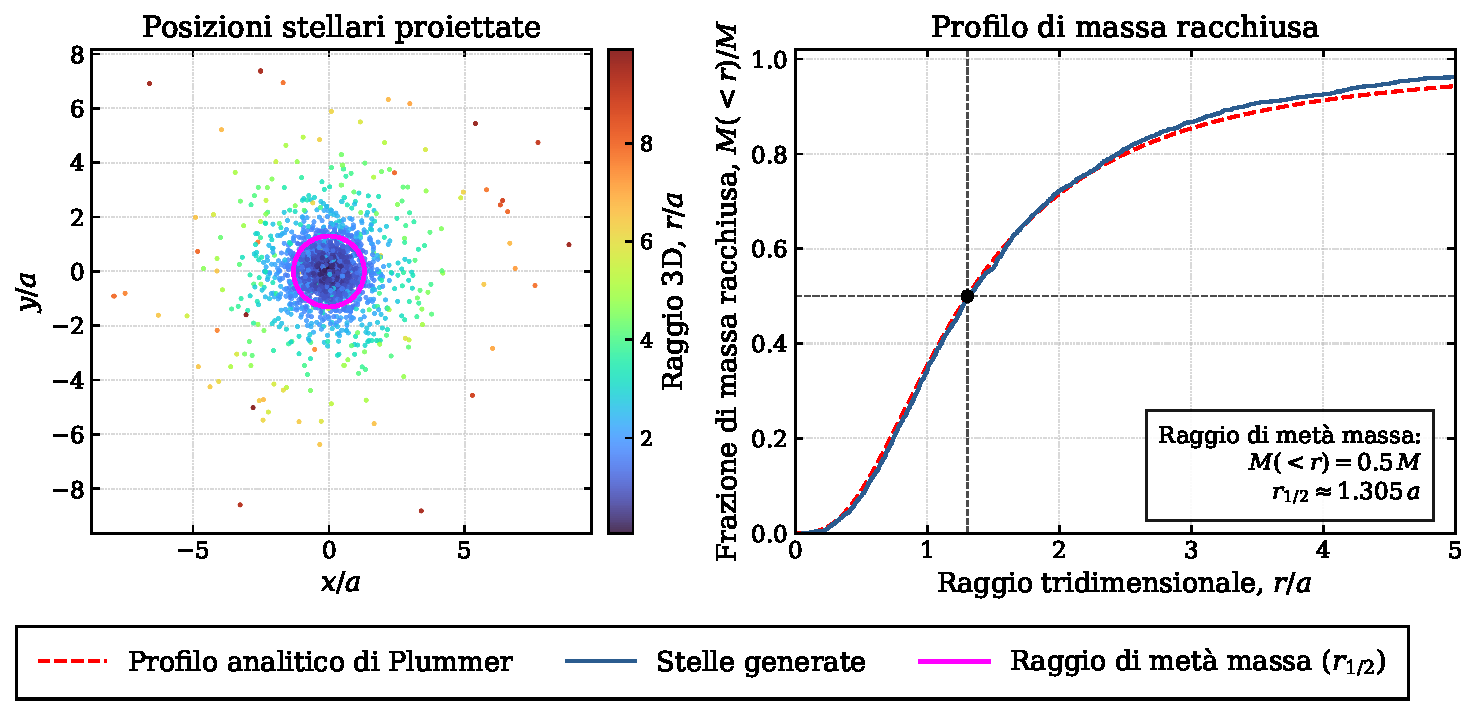
\includegraphics[width=0.8\textwidth]{./plots/initial_positions.pdf}
	\caption[Distribuzione spaziale iniziale del cluster]{Distribuzione tridimensionale delle posizioni iniziali delle stelle generate secondo il modello di Plummer ($N = 20000$, $\clusterRadius = 1.0$).}
	\label{fig:initial-positions}
\end{figure}

\subsection{Distribuzione delle velocità}
\label{subsec:velocita-iniziali}
Alle posizioni iniziali vengono associate velocità coerenti con il modello dinamico dell'ammasso. Assumendo che il potenziale gravitazionale sia nullo all'infinito, la velocità di fuga è definita come:
\begin{equation}
	\escapeVelocity(\radialDistance)
	=
	\sqrt{-2\potentialPhi(\radialDistance)}
	=
	\sqrt{\frac{2\gravitationalConstant\totalMass}
		{\sqrt{\radialDistance^2+\clusterRadius^2}}}.
	\label{eq:plummer-escape-velocity}
\end{equation}
Per il modello isotropo di Plummer, il modulo della velocità segue teoricamente la distribuzione \cite{eddington1916}:
\begin{equation}
	p(\velV \mid \radialDistance) \propto
	\velV^2
	\left(1-\frac{\velV^2}{\escapeVelocity(\radialDistance)^2}\right)^{7/2},
	\qquad
	0 \leq \velV < \escapeVelocity(\radialDistance).
	\label{eq:plummer-velocity-distribution}
\end{equation}
In alternativa al campionamento diretto di questa distribuzione, la dispersione delle velocità può essere ricavata dall'equazione di Jeans per un sistema sferico isotropo \cite{binneytremaine2008}:
\begin{equation}
	\frac{d\left[\densityRho(\radialDistance)
		\sigma_r^2(\radialDistance)\right]}{d\radialDistance}
	=
	-\densityRho(\radialDistance)
	\frac{d\potentialPhi(\radialDistance)}{d\radialDistance}.
	\label{eq:isotropic-jeans-equation}
\end{equation}
Per il modello di Plummer, la soluzione analitica è:
\begin{equation}
	\sigma_r^2(\radialDistance)
	=
	\frac{\gravitationalConstant\totalMass}
	{6\sqrt{\radialDistance^2+\clusterRadius^2}}.
	\label{eq:plummer-velocity-dispersion}
\end{equation}
In questo lavoro si utilizza la dispersione ricavata dall'equazione di Jeans per generare le componenti radiale e tangenziali della velocità mediante campionamento gaussiano. Questa scelta consente di costruire un metodo di campionamento basato sulla dispersione locale, da confrontare con il campionamento diretto della distribuzione teorica. Le particelle con energia specifica non negativa vengono scartate e le velocità sono infine riscalate per ottenere l'equilibrio viriale iniziale, come descritto nella Sezione~\ref{subsec:riscalamento-velocita}.

\begin{figure}[htbp]
	\centering
	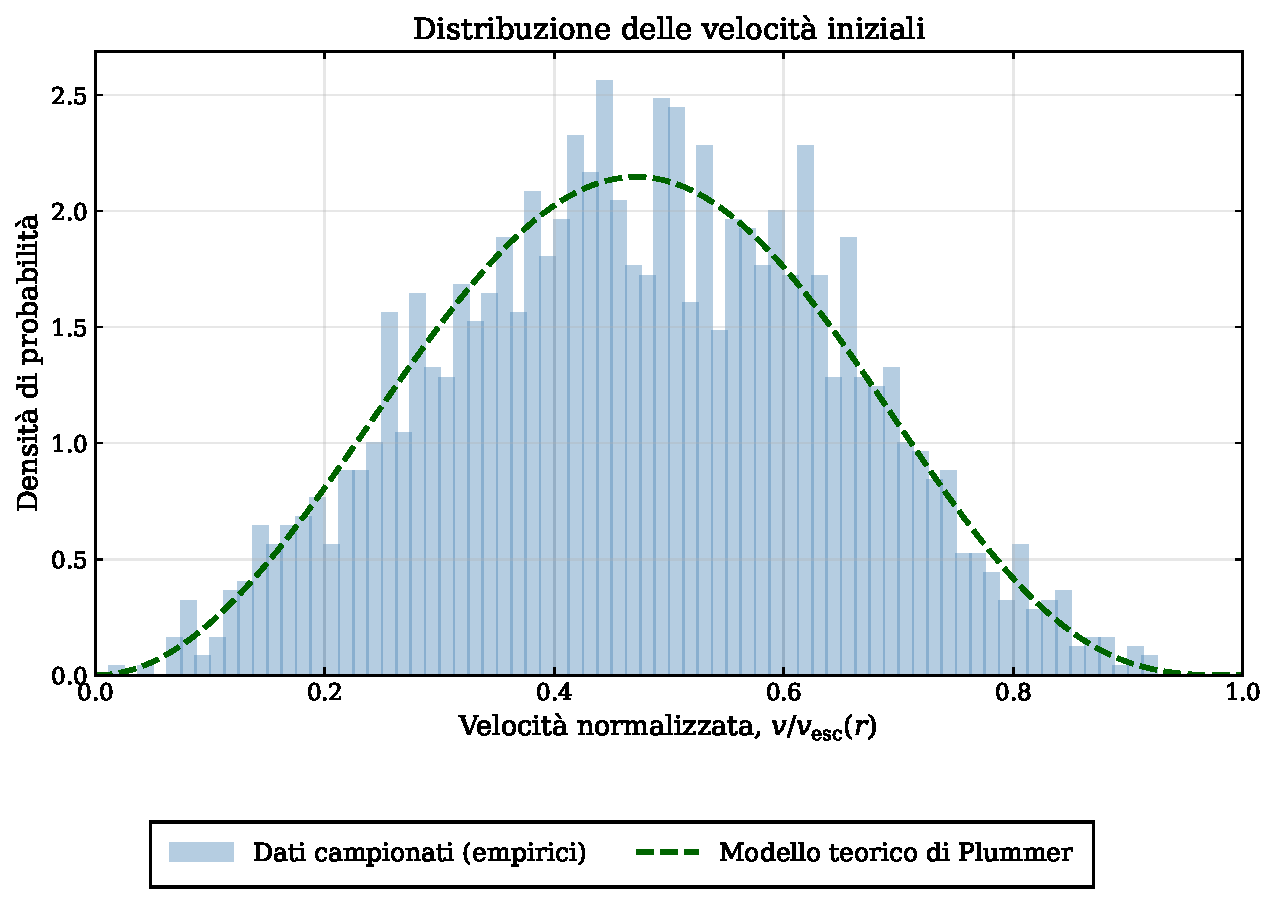
\includegraphics[width=0.6\textwidth]{./plots/velocity_distribution_comparison.pdf}
	\caption[Confronto tra le distribuzioni delle velocità iniziali]{Distribuzioni delle velocità normalizzate rispetto alla velocità locale di fuga\\($\numberOfStars = 20000$, $\clusterRadius = 1.0$).}
	\label{fig:velocity-distribution-comparison}
\end{figure}

\subsection{Condizione di equilibrio viriale}
\label{subsec:equilibrio-viriale}
Per valutare l'equilibrio dinamico iniziale dell'ammasso si considerano l'energia cinetica totale $\totalCineticEnergy$ e l'energia potenziale gravitazionale $\totalPotentialEnergy$ \cite{binneytremaine2008}. L'energia cinetica è data dalla somma dei contributi di tutte le stelle \cite{ciotti2021}:
\begin{equation}
	\totalCineticEnergy =
	\sum_{i=1}^{N} \frac{1}{2} m_i |\velV_i|^2,
	\label{eq:total-kinetic-energy}
\end{equation}
mentre l'energia potenziale gravitazionale è ottenuta sommando le interazioni tra tutte le coppie di stelle \cite{ciotti2021}:
\begin{equation}
	\totalPotentialEnergy =
	-\sum_{i=1}^{N-1}\sum_{j=i+1}^{N}
	\frac{\gravitationalConstant m_i m_j}
	{|\mathbf{x}_i-\mathbf{x}_j|}.
	\label{eq:total-potential-energy}
\end{equation}
Per un sistema autogravitante in equilibrio viriale, le due energie soddisfano la relazione \cite{ciotti2021}:
\begin{equation}
	2\totalCineticEnergy + \totalPotentialEnergy = 0.
	\label{eq:virial-equilibrium}
\end{equation}
Il rapporto viriale permette di quantificare lo scostamento da questa condizione:
\begin{equation}
	\virialRatio =
	\frac{2\totalCineticEnergy}
	{|\totalPotentialEnergy|}.
	\label{eq:virial-ratio}
\end{equation}
Il valore $\virialRatio=1$ corrisponde alla condizione viriale. Quando il rapporto calcolato dalle condizioni iniziali differisce da uno, è possibile correggerlo riscalando uniformemente le velocità, senza modificare le posizioni delle stelle.

\subsection{Riscalamento delle velocità}
\label{subsec:riscalamento-velocita}
Il campionamento delle velocità non garantisce che il rapporto viriale iniziale sia unitario. Per correggere questo scostamento, tutte le velocità vengono moltiplicate per un fattore comune $\velocityRescalingFactor$. L'energia cinetica risultante è:
\begin{equation}
	\totalCineticEnergy' =
	\velocityRescalingFactor^2 \totalCineticEnergy.
	\label{eq:rescaled-kinetic-energy}
\end{equation}
Poiché le posizioni rimangono invariate, anche l'energia potenziale resta costante durante questa operazione. Il rapporto viriale dopo il riscalamento è quindi:
\begin{equation}
	\virialRatio' =
	\velocityRescalingFactor^2 \virialRatio.
	\label{eq:rescaled-virial-ratio}
\end{equation}
Imponendo $\virialRatio'=1$, si ricava il fattore di riscalamento:
\begin{equation}
	\velocityRescalingFactor =
	\sqrt{\frac{|\totalPotentialEnergy|}
		{2\totalCineticEnergy}}
	=
	\frac{1}{\sqrt{\virialRatio}}.
	\label{eq:velocity-rescaling-factor}
\end{equation}
Il fattore viene calcolato a partire dalle energie del sistema e applicato a tutte le velocità. In questo modo si impone il rapporto viriale unitario per la configurazione iniziale, senza alterarne la distribuzione spaziale. Questa correzione riguarda il bilancio energetico globale e non garantisce, da sola, che la distribuzione delle velocità coincida con quella teorica del modello di Plummer.

\begin{figure}[htbp]
	\centering
	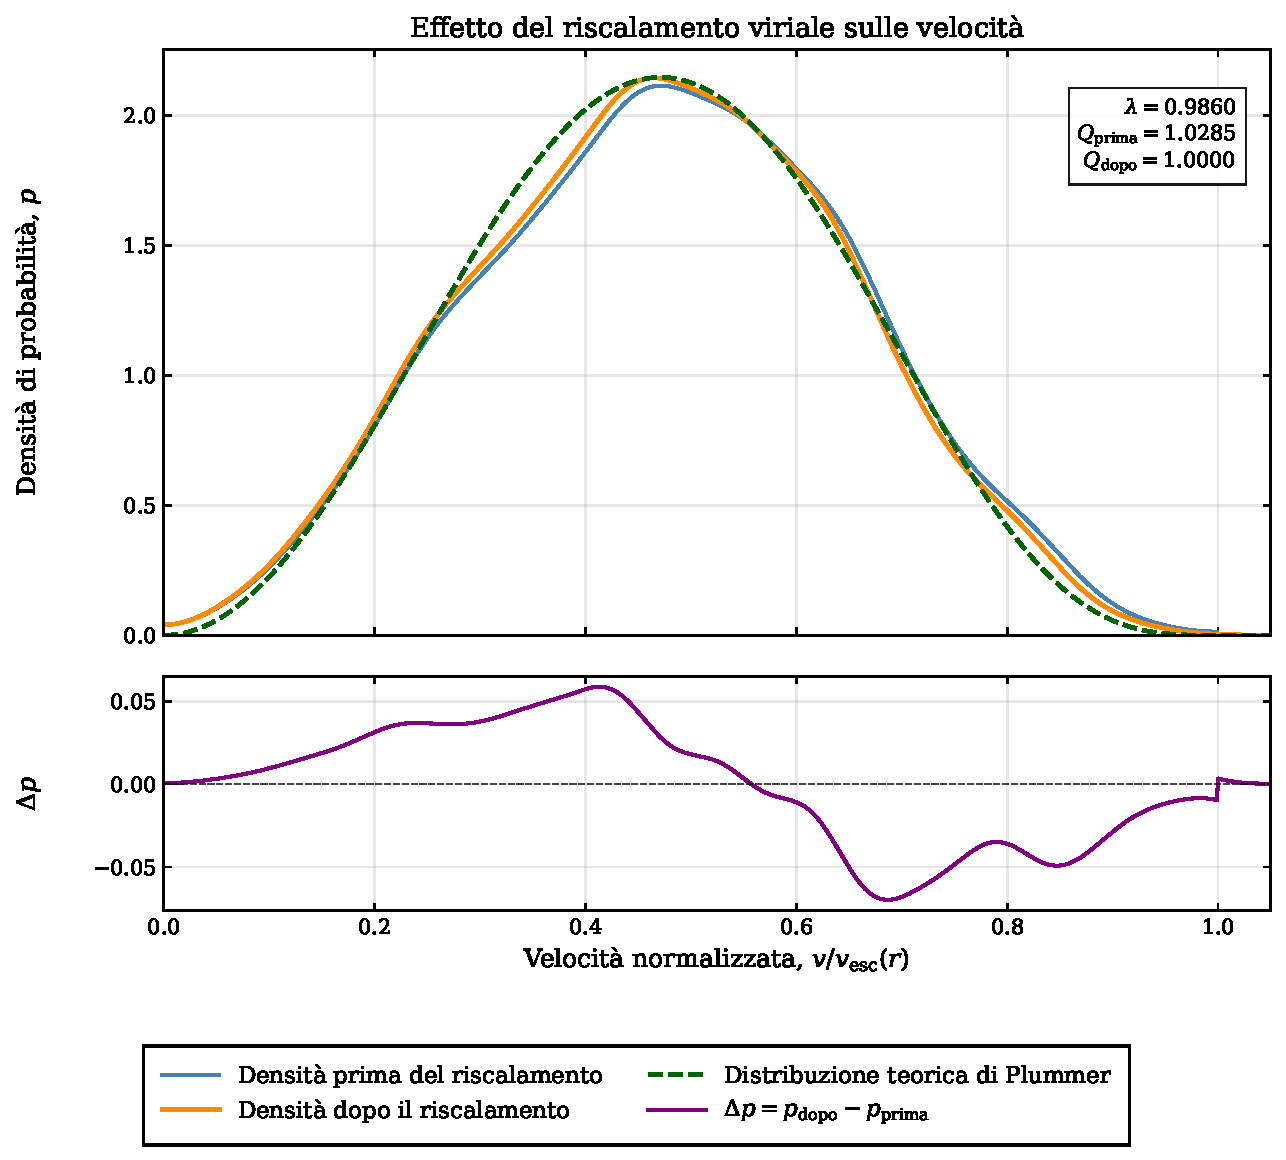
\includegraphics[width=0.6\textwidth]{./plots/velocity_rescaling.pdf}
	\caption[Confronto tra le distribuzioni delle velocità e diagnostica del viriale]{Confronto tra le distribuzioni delle velocità normalizzate ($\numberOfStars = 20000$, $\clusterRadius = 1.0$).}
	\label{fig:velocity-rescaling}
\end{figure}
\section{Evoluzione e dinamica orbitale}
\label{sec:evoluzione-ammasso}
L'evoluzione dell'ammasso stellare è descritta attraverso l'interazione gravitazionale tra le stelle e il potenziale galattico esterno, che ne determina la dinamica orbitale e l'evoluzione nel tempo.
\subsection{Potenziale galattico di Plummer}
\label{subsec:plummer-galattico}
Il potenziale gravitazionale adottato è quello di Plummer
\cite{plummer1911}, espresso in funzione della distanza $\galaxyDistance$
dal centro della galassia:
\begin{equation}
	\potentialPhi_{\mathrm{gal}}(\galaxyDistance) =
	-\frac{\gravitationalConstant \galaxyMass}
	{\sqrt{\galaxyDistance^2+\galaxyParameter^2}}
	\label{eq:galactic-plummer-potential}
\end{equation}
La forma adottata evita la singolarità del potenziale al centro,
presente nel caso di una massa puntiforme.\\
A partire dal potenziale definito nell'equazione~\eqref{eq:galactic-plummer-potential}, l'accelerazione gravitazionale esercitata dalla galassia si ottiene calcolando il gradiente del potenziale con segno opposto:
\begin{equation}
	\mathbf{a}_{\mathrm{gal}}(\mathbf{R}) =
	-\frac{\gravitationalConstant \galaxyMass}
	{(\galaxyDistance^2+\galaxyParameter^2)^{3/2}}\mathbf{R}
	\label{eq:galactic-plummer-acceleration}
\end{equation}
\begin{figure}[htbp]
	\centering
	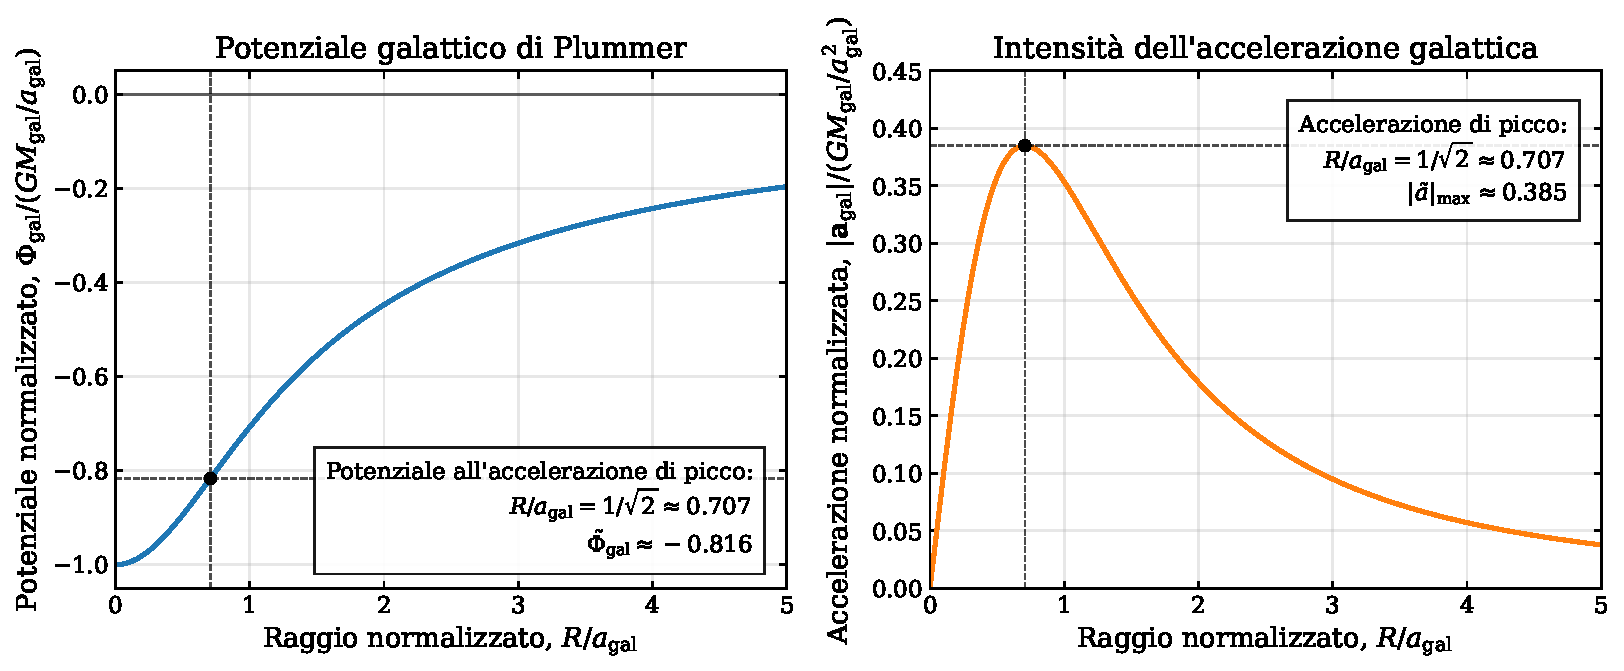
\includegraphics[width=\textwidth]{plots/galactic_plummer_potential.pdf}
	\caption{Potenziale gravitazionale e modulo dell'accelerazione del modello galattico di Plummer.}
	\label{fig:galactic-plummer}
\end{figure}

\subsection{Parametri orbitali}
\label{subsec:parametri-orbitali}
L'orbita iniziale dell'ammasso stellare viene definita attraverso il semiasse maggiore $\semiMajorAxis$ e l'eccentricità $\orbitEccentricity$. Nel caso kepleriano, questi parametri determinano le distanze di apocentro e pericentro secondo le relazioni:
\begin{equation}
	R_{\mathrm{apo}} = \semiMajorAxis(1+\orbitEccentricity),
	\qquad
	R_{\mathrm{peri}} = \semiMajorAxis(1-\orbitEccentricity)
	\label{eq:orbital-extrema}
\end{equation}
Nel modello adottato, tuttavia, il potenziale galattico è descritto dal modello di Plummer, che differisce dal potenziale kepleriano. Di conseguenza, le relazioni precedenti vengono utilizzate come scelta implementativa per determinare le distanze apsidali desiderate, senza assumere che la traiettoria risultante sia un'ellisse kepleriana.
Una volta determinate queste distanze, l'ammasso viene inizialmente collocato all'apocentro, dove la velocità è perpendicolare alla direzione radiale. Il suo modulo viene calcolato imponendo che apocentro e pericentro appartengano alla stessa orbita nel potenziale galattico adottato.
A questo scopo, si utilizzano la conservazione dell'energia meccanica specifica e del momento angolare specifico:\cite{goldstein2002}
\begin{equation}
	E = \frac{\velV^2}{2} + \potentialPhi_{\mathrm{gal}}(\radialDistance),
	\qquad
	L = \radialDistance v_{\mathrm{t}}
	\label{eq:orbital-conservation}
\end{equation}
dove $\velV$ è il modulo della velocità, $v_{\mathrm{t}}$ la sua componente tangenziale e $L$ il momento angolare specifico. In corrispondenza dell'apocentro e del pericentro, la velocità è interamente tangenziale. Uguagliando l'energia nei due punti e utilizzando la conservazione del momento angolare, si ottiene:
\begin{equation}
	L^2 =
	\frac{2\left[
		\potentialPhi_{\mathrm{gal}}(R_{\mathrm{apo}})
		-\potentialPhi_{\mathrm{gal}}(R_{\mathrm{peri}})
		\right]}
	{R_{\mathrm{peri}}^{-2}-R_{\mathrm{apo}}^{-2}}
	\label{eq:orbital-angular-momentum}
\end{equation}
Il modulo della velocità iniziale all'apocentro si ricava quindi da:
\begin{equation}
	v_{\mathrm{apo}} = \frac{L}{R_{\mathrm{apo}}}
	\label{eq:orbital-apocenter-velocity}
\end{equation}
Poiché l'approssimazione kepleriana risulta incoerente con un potenziale galattico esteso, la velocità iniziale viene ricavata rigorosamente dal potenziale di Plummer e dalle distanze apsidali, preservando la coerenza energetica del sistema. L'effetto di questa scelta è visibile in Figura~\ref{fig:orbital-methods-comparison}.
\begin{figure}[htbp]
	\centering
	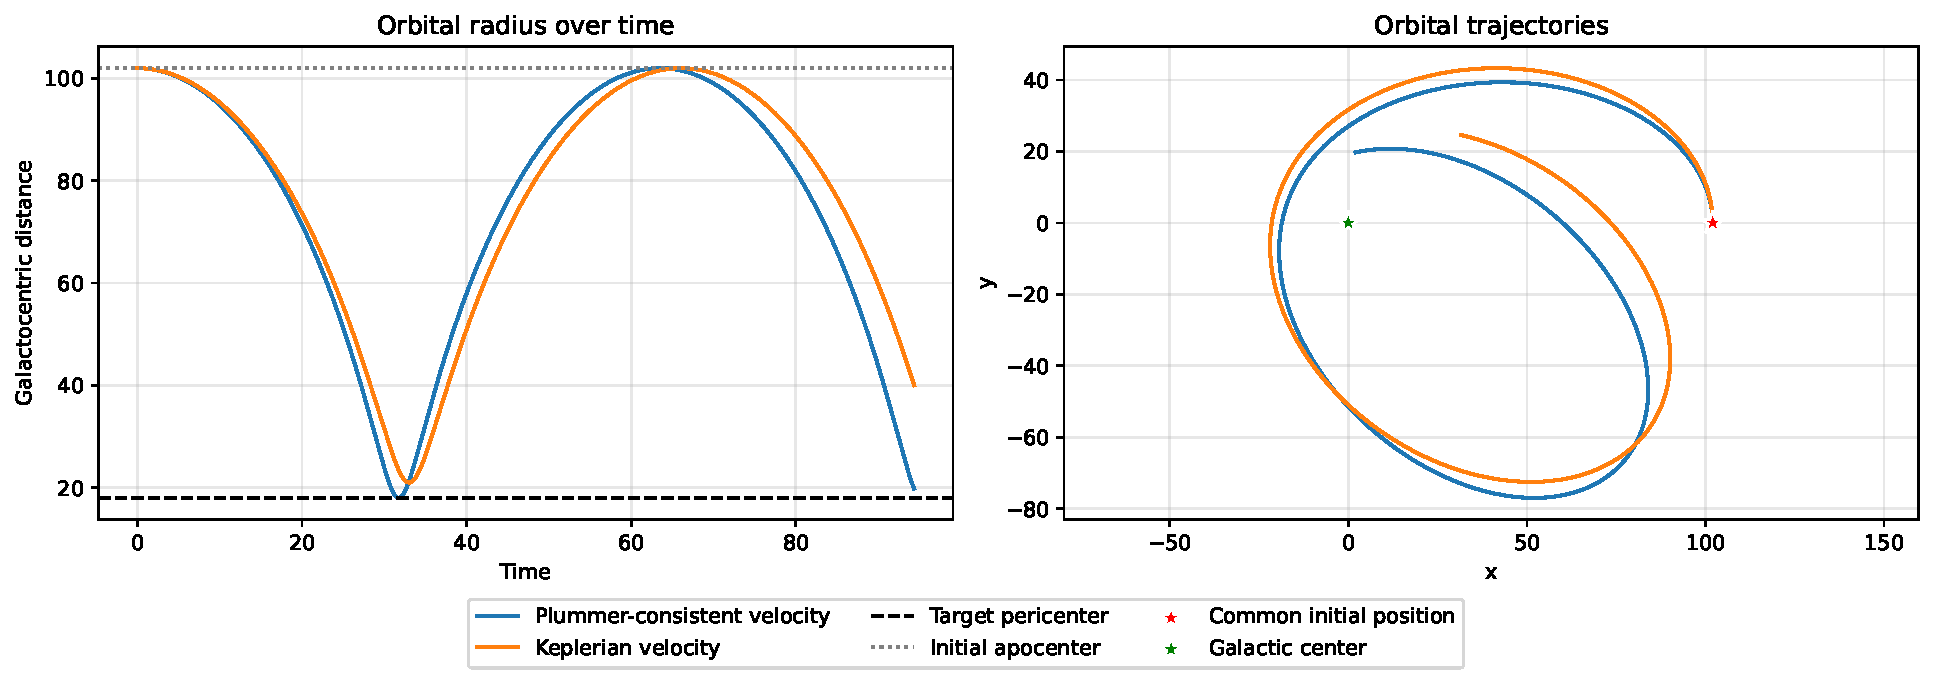
\includegraphics[width=\textwidth]{./plots/orbital_methods_comparison.pdf}
	\caption[Confronto tra i metodi di calcolo della velocità orbitale]{Confronto tra le due orbite fino al $50\%$ di divergenza del semiasse maggiore.\\($\galaxyMass = 2000.0$, $\galaxyRadius = 10.0$, $\gravitationalConstant = 1.0$, $\semiMajorAxis = 60.0$, $\orbitEccentricity = 0.7$, $\Delta t = 0.001$, Leapfrog).}
	\label{fig:orbital-methods-comparison}
\end{figure}

\subsection{Equazioni del moto}
\label{subsec:equazioni-moto}
L'evoluzione dell'ammasso stellare è descritta dalle equazioni di Newton per un sistema di particelle gravitazionalmente interagenti. Indicando con $\mathbf{x}_i$ la posizione della stella $i$ e con $m_i$ la sua massa, le equazioni del moto sono:
\begin{equation}
	\frac{d\mathbf{x}_i}{dt} = \mathbf{v}_i,
	\qquad
	\frac{d\mathbf{v}_i}{dt} = \mathbf{a}_i
	\label{eq:equations-of-motion}
\end{equation}
L'accelerazione di ciascuna stella riceve due contributi: l'interazione gravitazionale con le altre stelle dell'ammasso e il campo esterno generato dalla galassia. Nel caso newtoniano, il contributo interno è espresso da:
\begin{equation}
	\mathbf{a}_{i,\mathrm{int}} =
	-G\sum_{\substack{j=1\\j\neq i}}^N
	m_j
	\frac{\mathbf{x}_i-\mathbf{x}_j}
	{|\mathbf{x}_i-\mathbf{x}_j|^3}
	\label{eq:internal-gravitational-acceleration}
\end{equation}
L'accelerazione totale è quindi la somma del contributo interno e di quello galattico definito nella Sezione~\ref{subsec:plummer-galattico}:
\begin{equation}
	\mathbf{a}_i =
	\mathbf{a}_{i,\mathrm{int}} +
	\mathbf{a}_{\mathrm{gal}}(\mathbf{x}_i)
	\label{eq:total-acceleration}
\end{equation}
Questa formulazione permette di descrivere simultaneamente la dinamica interna dell'ammasso e la sua risposta al campo gravitazionale esterno. Le interazioni reciproche determinano l'evoluzione della struttura stellare, mentre il potenziale galattico influenza il moto complessivo dell'ammasso e può favorire la perdita di stelle gravitazionalmente non più legate alla sua componente interna \cite{binneytremaine2008}.

\subsection{Integrazione numerica}
\label{subsec:integrazione-numerica}
L'evoluzione gravitazionale di un ammasso composto da migliaia di stelle richiede l'integrazione numerica delle equazioni del moto. Per individuare un compromesso tra accuratezza e costo computazionale, sono stati confrontati diversi metodi di integrazione, con particolare attenzione allo schema \emph{leapfrog} e all'integratore adattivo IAS15 \cite{hairer2006geometric,rein2015ias15}.
Il metodo leapfrog, nella formulazione \emph{kick-drift-kick}, è un integratore simplettico del secondo ordine, adatto alle simulazioni dinamiche a lungo termine\cite{quinn1997timestepping}.\\
Indicando con $\deltat$ il passo temporale, l'aggiornamento delle posizioni e delle velocità è descritto da:\\
\begin{align}
	\mathbf{v}_{i}^{n+1/2}
	&= \mathbf{v}_{i}^{n}
	+ \frac{\deltat}{2}\mathbf{a}_{i}^{n}\\
	\mathbf{x}_{i}^{n+1}
	&= \mathbf{x}_{i}^{n}
	+ \deltat\,\mathbf{v}_{i}^{n+1/2}\\
	\mathbf{v}_{i}^{n+1}
	&= \mathbf{v}_{i}^{n+1/2}
	+ \frac{\deltat}{2}\mathbf{a}_{i}^{n+1}
	\label{eq:leapfrog-update}
\end{align}
Le prestazioni dei diversi metodi e dei passi temporali $\deltat=0.01$ e $\deltat=0.001$ vengono valutate attraverso l'errore relativo dell'energia totale, utilizzando IAS15 come riferimento ad alta precisione. Il confronto consente di quantificare l'errore introdotto dall'integrazione e di individuare il passo temporale più adeguato alle simulazioni successive.
METTERE GRAFICO QUI CONFRONTO ERRORI TRA LEAPFROG E IAS15

\subsection{Centro di massa percentile}
\label{subsec:com-percentile}
Il centro di massa globale può essere influenzato dalle stelle periferiche, soprattutto durante lo stripping mareale. Per ottenere una stima più rappresentativa della regione centrale dell'ammasso, viene introdotto un metodo basato su selezioni percentilari successive, riconducibile ai principi delle stime robuste \cite{wilcox2023guide}.
A partire dal centro di massa globale $\mathbf{x}_{\mathrm{COM}}^{(0)}$, si calcolano le distanze delle singole stelle:
\begin{equation}
	d_i^{(k)} = \left|\mathbf{x}_i-\mathbf{x}_{\mathrm{COM}}^{(k)}\right|
	\label{eq:com-percentile-distance}
\end{equation}
A ogni passaggio si mantiene la frazione più centrale del campione, ricalcolando il centro come media pesata sulle masse:
\begin{equation}
	\mathbf{x}_{\mathrm{COM}}^{(k+1)} =
	\frac{\displaystyle\sum_{i\in S_q^{(k)}}m_i\mathbf{x}_i}
	{\displaystyle\sum_{i\in S_q^{(k)}}m_i}
	\label{eq:com-percentile}
\end{equation}
La selezione utilizza in successione i percentili $80$, $65$, $50$, $35$ e $20$, interrompendosi quando rimangono meno di cinque stelle. La stessa procedura, applicata alle velocità, consente di stimare il moto del centro. La coordinata $y$ del centro percentile viene infine utilizzata per contare le orbite completate, identificando gli attraversamenti di $y=0$ dal semipiano negativo a quello non negativo.\\
Gli effetti di questa correzione sono visibili in Figura~\ref{fig:com-trajectories}, dove, già dopo una prima orbita, le due stime mostrano una divergenza attribuibile all'influenza delle stelle periferiche sul centro di massa globale.
\begin{figure}[htbp]
	\centering
	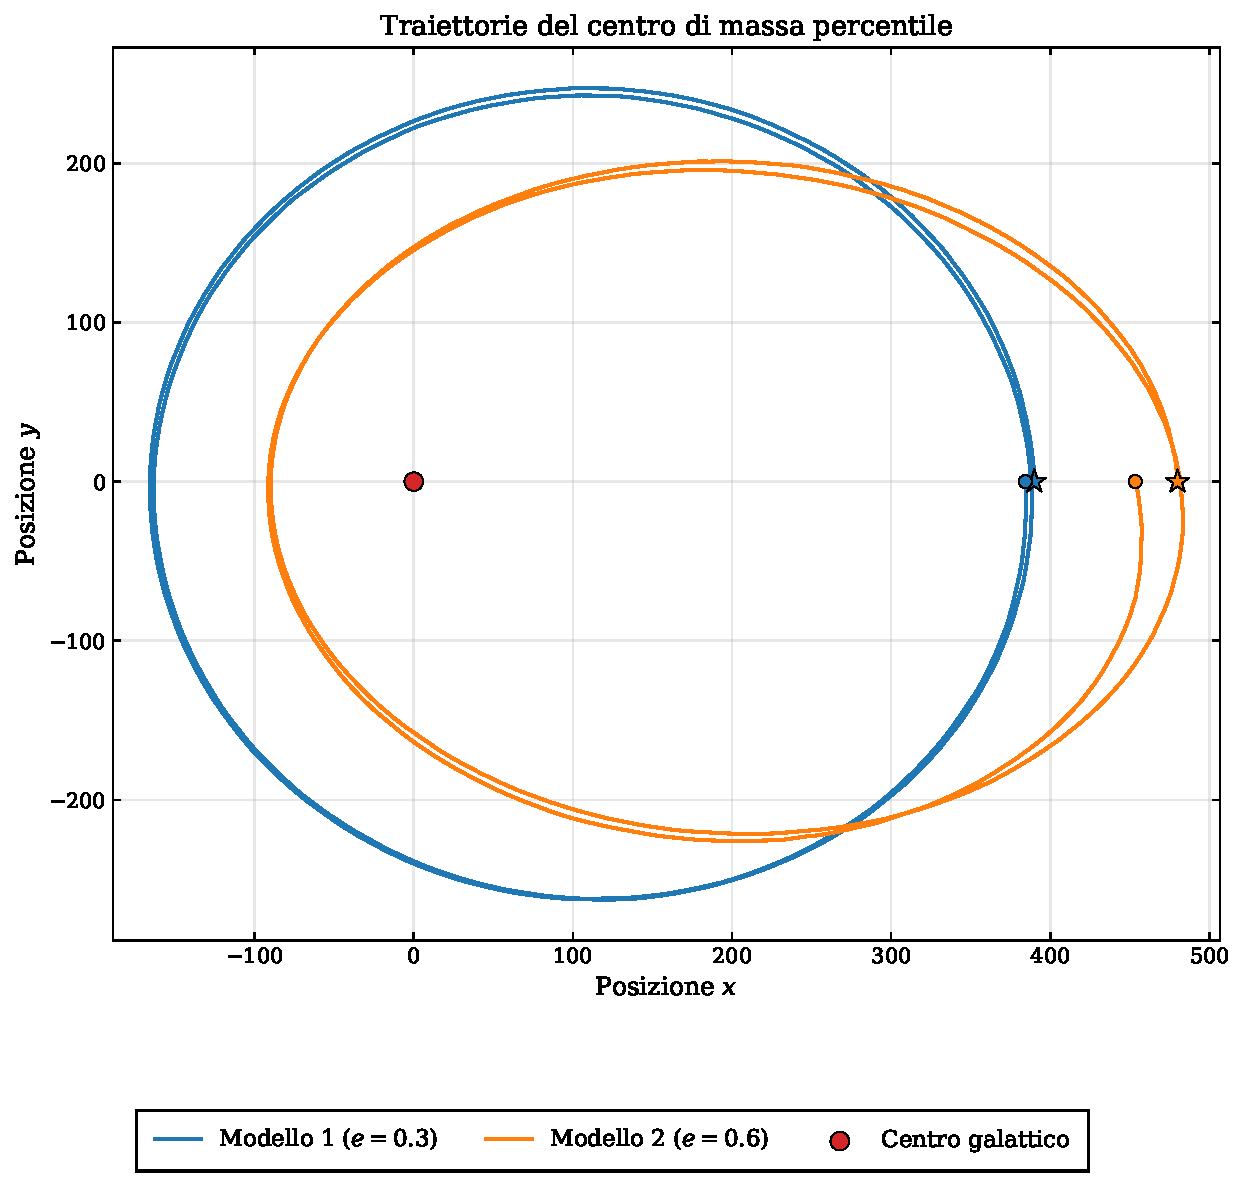
\includegraphics[width=\textwidth]{./plots/com_trajectories.pdf}
	\caption[Traiettorie del centro di massa classico e percentile]{Traiettorie di due orbite del centro di massa classico e percentile.\\($\numberOfStars = 2000$, $\clusterRadius = 1.0$, $\galaxyMass = 2000.0$, $\galaxyRadius = 10.0$, $\gravitationalConstant = 1.0$, $\semiMajorAxis = 294.0$, $\orbitEccentricity = 0.7$, $\deltat = 0.001$, Leapfrog)}
	\label{fig:com-trajectories}
\end{figure}

      \chapter{Dataset e Machine Learning}


\section{Generazione del dataset}
\label{sec:costruzione-dataset}
Per ottenere un dataset affidabile, è necessario definire i parametri delle simulazioni, stabilendo quali mantenere costanti e quali variare. Questa scelta permette di studiare come le condizioni orbitali influenzino l'evoluzione degli ammassi stellari, mantenendo invariate le altre caratteristiche del sistema.
\subsection{Parametri dell'ammasso stellare}
\label{subsec:condizioni-iniziali}
L'ammasso stellare viene inizializzato secondo il modello di Plummer, descritto nella Sezione~\ref{subsec:plummer}. In tutte le simulazioni vengono fissati il numero di stelle, $\numberOfStars=200$, il parametro di scala $\clusterRadius=1.0$ e la massa totale $\totalMass=1.0$.\\
Le stelle hanno tutte la stessa massa, calcolata come:
\begin{equation}
	\starMass=\frac{\totalMass}{\numberOfStars}=0.005.
	\label{eq:massa-singola-stella}
\end{equation}
Per ottenere diverse realizzazioni iniziali dell'ammasso vengono utilizzati 15 semi di generazione distinti, che determinano differenti distribuzioni iniziali delle posizioni e delle velocità stellari. In questo modo è possibile valutare l'influenza delle condizioni iniziali sui risultati, evitando di basare l'analisi su una singola realizzazione dell'ammasso.
\subsection{Parametri galattici ed orbitali}
\label{subsec:parametri-orbitali}
Il potenziale gravitazionale esterno è descritto dal modello di Plummer, introdotto nella Sezione~\ref{subsec:plummer-galattico}, con massa galattica $\galaxyMass=3000.0$ e parametro di scala $\galaxyRadius=20.0$, mantenuti costanti in tutte le simulazioni.
Le orbite sono definite mediante il semiasse maggiore $\semiMajorAxis$ e l'eccentricità $\orbitEccentricity$. Il primo assume 30 valori compresi tra $10.0$ e $300.0$, con incrementi di $10.0$:
\[
\semiMajorAxis \in \{10,20,30,\ldots,290,300\}.
\]
L'eccentricità assume invece 38 valori compresi tra $0.0$ e $0.925$, con incrementi di $0.025$:
\[
\orbitEccentricity \in \{0,0.025,0.050,\ldots,0.900,0.925\}.
\]
Considerando tutte le combinazioni dei due parametri, si ottengono $30\times38=1140$ configurazioni orbitali. Ciascuna viene utilizzata per diverse realizzazioni iniziali dell'ammasso, così da studiare l'evoluzione del sistema al variare delle dimensioni e della forma dell'orbita.
\subsection{Parametri di integrazione}
\label{subsec:parametri-integrazione}
Le simulazioni adottano una costante gravitazionale $\gravitationalConstant=1.0$, scelta che consente di esprimere tutte le grandezze in un sistema di unità coerente, evitando conversioni tra diverse unità di misura. L'integrazione numerica viene eseguita con il metodo leapfrog \cite{hairer2006geometric}, utilizzando un passo temporale $\deltat=0.005$. Per regolarizzare il potenziale gravitazionale durante gli incontri ravvicinati tra le stelle, viene adottato un parametro di ammorbidimento pari a $\softeningLength=0.01$.
Il tempo finale delle simulazioni è fissato a $\simulationEndTime=700.0$, per contenere l'influenza della dissoluzione dell'ammasso dovuta alla sua evoluzione dinamica interna e concentrarsi sugli effetti della rimozione mareale galattica \cite{cai2016evolution}.
\subsection{Riepilogo dei parametri}
\label{subsec:riepilogo-parametri}
La Tabella~\ref{tab:parametri-dataset} riassume i parametri adottati per le simulazioni, distinguendo quelli mantenuti costanti da quelli variati per esplorare le diverse configurazioni orbitali.
\begin{table}[htbp]
	\centering
	\caption{Parametri adottati per la generazione del dataset.}
	\label{tab:parametri-dataset}
	\begin{tabular}{lll}
		\hline
		\textbf{Parametro} & \textbf{Simbolo} & \textbf{Valore} \\
		\hline
		\multicolumn{3}{l}{\textit{Ammasso stellare}} \\
		Numero di stelle & $\numberOfStars$ & $200$ \\
		Massa totale & $\totalMass$ & $1.0$ \\
		Massa di una stella & $\starMass$ & $0.005$ \\
		Parametro di scala del modello di Plummer & $\clusterRadius$ & $1.0$ \\
		Numero di semi generativi utilizzati & --- & $15$ \\
		\hline
		\multicolumn{3}{l}{\textit{Potenziale galattico}} \\
		Massa galattica & $\galaxyMass$ & $3000.0$ \\
		Parametro di scala galattico & $\galaxyRadius$ & $20.0$ \\
		\hline
		\multicolumn{3}{l}{\textit{Parametri orbitali}} \\
		Semiasse maggiore & $\semiMajorAxis$ & $[10.0,\,300.0]$, passo $10.0$ \\
		Eccentricità & $\orbitEccentricity$ & $[0.0,\,0.925]$, passo $0.025$ \\
		\hline
		\multicolumn{3}{l}{\textit{Integrazione numerica}} \\
		Costante gravitazionale & $\gravitationalConstant$ & $1.0$ \\
		Passo temporale & $\deltat$ & $0.005$ \\
		Parametro di ammorbidimento & $\softeningLength$ & $0.01$ \\
		Tempo finale & $\simulationEndTime$ & $700.0$ \\
		Integratore & --- & Leapfrog \\		
		\hline
	\end{tabular}
\end{table}
\section{Analisi del dataset}
\label{sec:analisi-dataset}
Come descritto nelle Sezioni~\ref{subsec:condizioni-iniziali} e~\ref{subsec:parametri-orbitali}, vengono considerate $15$ realizzazioni iniziali dell'ammasso, ciascuna evoluta per $1140$ configurazioni orbitali, ottenute combinando i $30$ valori del semiasse maggiore con i $38$ valori dell'eccentricità. Il dataset comprende quindi un totale di $15\times1140=17100$ simulazioni.
\subsection{Distribuzione delle grandezze finali}
\label{subsec:distribuzione-grandezze-finali}
Per analizzare i risultati delle simulazioni, vengono considerati gli istogrammi della frazione di massa legata finale $\boundMassFraction$ e del rapporto tra il raggio di metà massa finale e quello iniziale, definito come:
\[
\halfMassRadiusRatio=\frac{r_{1/2}}{r_{1/2,0}}
\]
\begin{figure}[htbp]
	\centering
	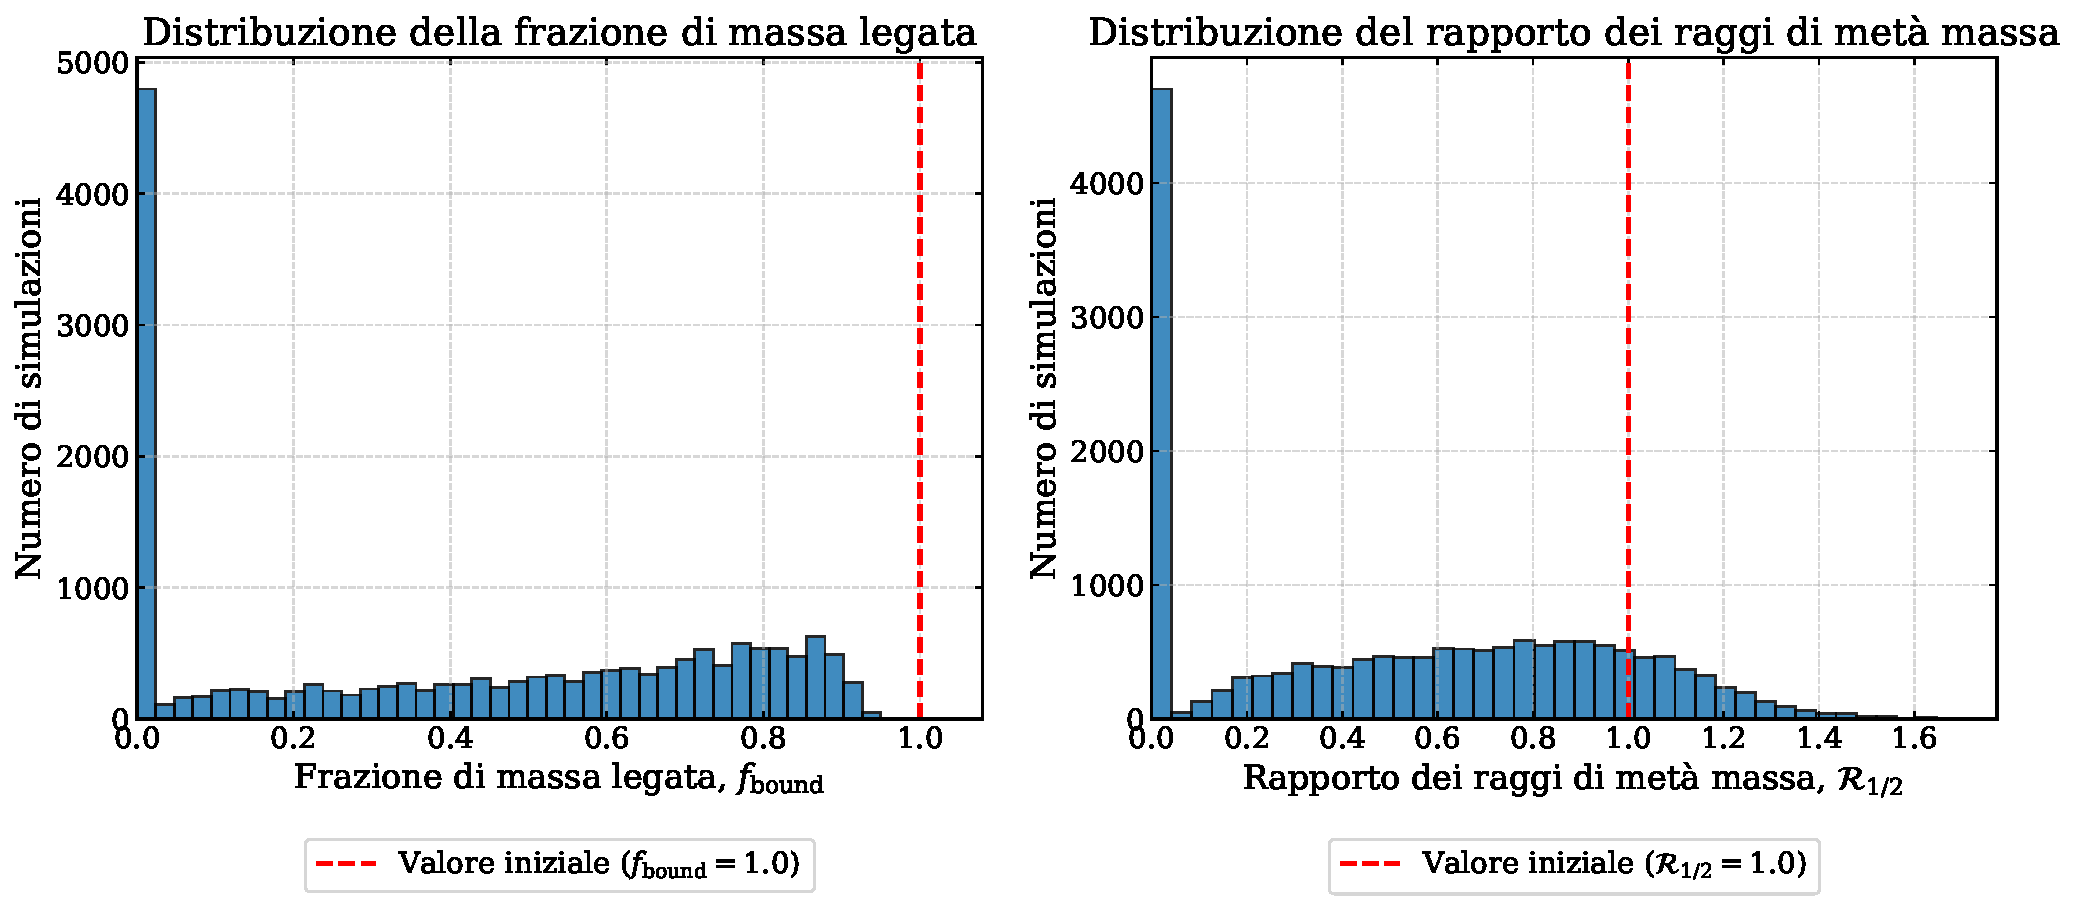
\includegraphics[width=\textwidth]{./plots/distribuzioni_bmf_hmr.pdf}
	\caption{Distribuzione della frazione di massa legata finale $\boundMassFraction$ (a sinistra) e del rapporto tra il raggio di metà massa finale e iniziale $\halfMassRadiusRatio$ (a destra).}
	\label{fig:distribuzione-grandezze-finali}
\end{figure}
Dalla figura~\ref{fig:distribuzione-grandezze-finali} si nota che entrambe le distribuzioni presentano un andamento bimodale, caratterizzato da due gruppi di valori distinti. Si osserva che in $4689$ simulazioni, pari al $27.42\%$ del dataset, sia la frazione di massa legata $\boundMassFraction$ sia il rapporto tra i raggi di metà massa $\halfMassRadiusRatio$ sono nulli. In questi casi, nessuna stella risulta più legata all'ammasso e le stelle si sono totalmente disperse sotto l'effetto delle forze mareali galattiche.
\subsection{Relazione tra parametri orbitali ed esiti delle simulazioni}
\label{subsec:relazione-parametri-esiti}
La Figura~\ref{fig:heatmap-bmf-hmr} mostra le mappe di calore della frazione di massa legata finale $\boundMassFraction$ e del raggio di metà massa finale $R_{1/2}$, in funzione del semiasse maggiore $\semiMajorAxis$ e dell'eccentricità $\orbitEccentricity$. Ogni cella rappresenta la media dei risultati delle $15$ realizzazioni iniziali per una determinata configurazione orbitale.
\begin{figure}[htbp]
	\centering
	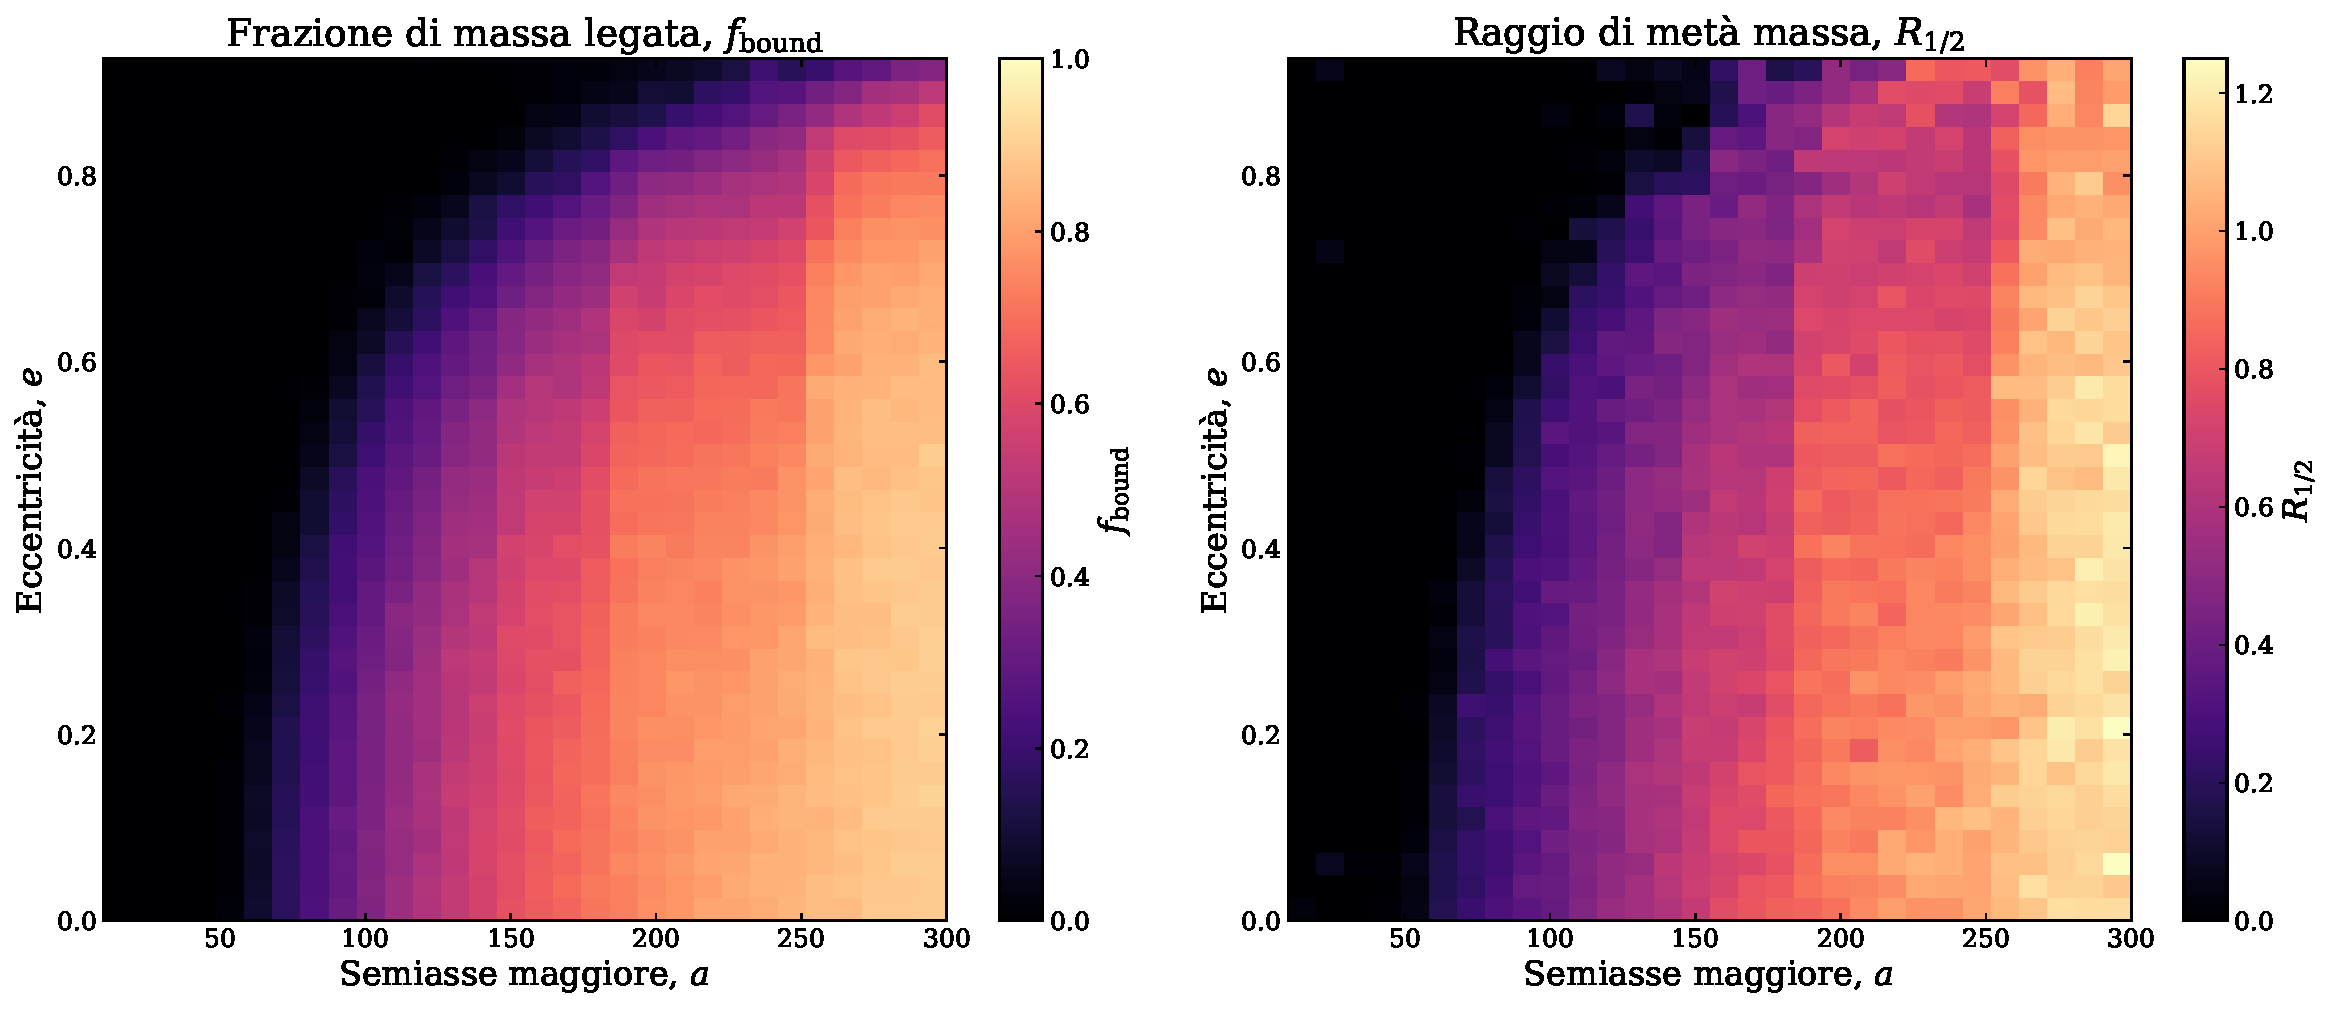
\includegraphics[width=\textwidth]{./plots/mappa_calore_bmf_hmr.pdf}
	\caption{Mappe di calore dei valori medi della frazione di massa legata finale $\boundMassFraction$ (a sinistra) e del raggio di metà massa finale $R_{1/2}$ (a destra), in funzione del semiasse maggiore $\semiMajorAxis$ e dell'eccentricità $\orbitEccentricity$.}
	\label{fig:heatmap-bmf-hmr}
\end{figure}
Le mappe mostrano che per valori del semiasse maggiore inferiori a circa $75$ l'ammasso subisce una dissoluzione completa, dovuta alla forte influenza del potenziale galattico. Anche l'eccentricità influisce sull'evoluzione dell'ammasso: all'aumentare di $\orbitEccentricity$, la dissoluzione diventa progressivamente più marcata, poiché l'ammasso si avvicina maggiormente alla galassia al pericentro, subendo effetti mareali più intensi.


\section{Definizione del problema di classificazione}
\subsection{Classificazione degli ammassi stellari}
\label{subsec:criterio-vivi-morti}
\subsection{Suddivisione in training set e test set}
\label{subsec:suddivisione-dataset}
Per valutare la capacità dei modelli di classificare simulazioni mai viste durante l'addestramento, il dataset viene suddiviso: l'80\% dei dati viene utilizzato per l'addestramento e il restante 20\% per la valutazione finale. La suddivisione è stratificata rispetto alla classe di appartenenza, ovvero viene mantenuta in entrambi gli insiemi la stessa proporzione di ammassi vivi e morti presente nel dataset completo.
\subsection{Standardizzazione delle variabili}
\label{subsec:standardizzazione-variabili}
Il semiasse maggiore e l'eccentricità hanno scale e distribuzioni differenti. Per i modelli sensibili alla scala delle variabili, vengono quindi standardizzati mediante la trasformazione
\[
x' = \frac{x-\mu}{\sigma},
\]
dove $x$ è il valore originale, mentre $\mu$ e $\sigma$ sono rispettivamente la media e la deviazione standard della variabile. Questi parametri vengono calcolati sul training set e utilizzati anche per trasformare il test set, in modo che la valutazione avvenga senza influenzare la fase di addestramento.
\subsection{Albero decisionale}
\label{subsec:albero-decisionale}
\subsection{Support Vector Machine}
\label{subsec:svm}
\subsection{Multi-Layer Perceptron}
\label{subsec:mlp}
\subsection{Regioni decisionali}
\label{subsec:regioni-decisionali}
\subsection{Confronto tramite F1-score}
\label{subsec:confronto-f1-score}
      \chapter{Conclusioni}
\label{cha:conclusioni}

      \chapter{Conclusioni}
\label{cha:conclusioni}
Dal confronto tra i due modelli emergono alcune differenze interessanti. L'SVC ha ottenuto risultati più limitati, ma permette di ricondurre la classificazione a un'equazione quadratica, rendendo esplicita la frontiera decisionale e quindi più facile da interpretare. L'MLP ha invece fornito risultati molto buoni: osservando la sua frontiera decisionale, si nota che ricalca molto da vicino la distribuzione degli esiti già visibile nelle mappe di calore della Sezione~\ref{subsec:relazione-parametri-esiti}.
Le difficoltà maggiori si incontrano nella zona di transizione tra sopravvivenza e dissoluzione, dove ammassi con gli stessi parametri orbitali possono avere esiti diversi a seconda della loro realizzazione iniziale. Questo potrebbe indicare che semiasse maggiore ed eccentricità, da soli, non siano sufficienti a descrivere il risultato. Sarebbe quindi interessante, in futuro, aumentare il numero di realizzazioni per ogni configurazione orbitale e includere altre grandezze diagnostiche tra i dati in ingresso, così da fornire ai modelli informazioni più complete.
Un'altra difficoltà emersa durante lo studio riguarda la dissoluzione autonoma degli ammassi, dovuta alla loro stessa evoluzione interna e non direttamente all'azione del potenziale galattico. Proprio per limitarne l'influenza, il tempo finale delle simulazioni è stato fissato a $T_{\mathrm{end}}=700$. Anche questo aspetto potrebbe essere approfondito in futuro, ad esempio aumentando il numero di stelle utilizzato per ciascun ammasso.
Un risultato positivo riguarda invece il modello di Plummer utilizzato per generare le condizioni iniziali. Sebbene la sua descrizione teorica sia formulata nel limite $N\to\infty$, si è dimostrato efficace anche con ammassi di sole 200 stelle. Il riscalamento delle velocità iniziali si è rivelato particolarmente importante per ottenere configurazioni in equilibrio viriale.
Infine, l'intervallo dei semiassi maggiori esplorato costituisce un altro limite del dataset. Sarebbe interessante ampliarlo e verificare se i modelli riescano a prevedere l'esito di configurazioni con parametri orbitali al di fuori degli intervalli utilizzati durante l'addestramento. In questo modo si potrebbe valutare la loro capacità di estrapolare le relazioni apprese e applicarle anche a configurazioni mai simulate in precedenza.
      
      
    \endgroup


    % bibliografia in formato bibtex
    %
    % aggiunta del capitolo nell'indice
    \addcontentsline{toc}{chapter}{Bibliografia}
    % stile con ordinamento alfabetico in funzione degli autori
    \bibliographystyle{plain}
    \bibliography{biblio}
%%%%%%%%%%%%%%%%%%%%%%%%%%%%%%%%%%%%%%%%%%%%%%%%%%%%%%%%%%%%%%%%%%%%%%%%%%
%%%%%%%%%%%%%%%%%%%%%%%%%%%%%%%%%%%%%%%%%%%%%%%%%%%%%%%%%%%%%%%%%%%%%%%%%%
%% Nota
%%%%%%%%%%%%%%%%%%%%%%%%%%%%%%%%%%%%%%%%%%%%%%%%%%%%%%%%%%%%%%%%%%%%%%%%%%
%% Nella bibliografia devono essere riportati tutte le fonti consultate 
%% per lo svolgimento della tesi. La bibliografia deve essere redatta 
%% in ordine alfabetico sul cognome del primo autore. 
%% 
%% La forma della citazione bibliografica va inserita secondo la fonte utilizzata:
%% 
%% LIBRI
%% Cognome e iniziale del nome autore/autori, la data di edizione, titolo, casa editrice, eventuale numero dell’edizione. 
%% 
%% ARTICOLI DI RIVISTA
%% Cognome e iniziale del nome autore/autori, titolo articolo, titolo rivista, volume, numero, numero di pagine.
%% 
%% ARTICOLI DI CONFERENZA
%% Cognome e iniziale del nome autore/autori (anno), titolo articolo, titolo conferenza, luogo della conferenza (città e paese), date della conferenza, numero di pagine. 
%% 
%% SITOGRAFIA
%% La sitografia contiene un elenco di indirizzi Web consultati e disposti in ordine alfabetico. 
%% E’ necessario:
%%   Copiare la URL (l’indirizzo web) specifica della pagina consultata
%%   Se disponibile, indicare il cognome e nome dell’autore, il titolo ed eventuale sottotitolo del testo
%%   Se disponibile, inserire la data di ultima consultazione della risorsa (gg/mm/aaaa).    
%%%%%%%%%%%%%%%%%%%%%%%%%%%%%%%%%%%%%%%%%%%%%%%%%%%%%%%%%%%%%%%%%%%%%%%%%%
%%%%%%%%%%%%%%%%%%%%%%%%%%%%%%%%%%%%%%%%%%%%%%%%%%%%%%%%%%%%%%%%%%%%%%%%%%
    

%    \titleformat{\chapter}
%        {\normalfont\Huge\bfseries}{Allegato \thechapter}{1em}{}
%    % sezione Allegati - opzionale
%    \appendix
%    \chapter{Titolo primo allegato}

Lorem ipsum dolor sit amet, consectetur adipiscing elit. Donec sed nunc orci. Aliquam nec nisl vitae sapien pulvinar dictum quis non urna. Suspendisse at dui a erat aliquam vestibulum. Quisque ultrices pellentesque pellentesque. Pellentesque egestas quam sed blandit tempus. Sed congue nec risus posuere euismod. Maecenas ut lacus id mauris sagittis egestas a eu dui. Class aptent taciti sociosqu ad litora torquent per conubia nostra, per inceptos himenaeos. Pellentesque at ultrices tellus. Ut eu purus eget sem iaculis ultricies sed non lorem. Curabitur gravida dui eget ex vestibulum venenatis. Phasellus gravida tellus velit, non eleifend justo lobortis eget. 

\section{Titolo}
Lorem ipsum dolor sit amet, consectetur adipiscing elit. Donec sed nunc orci. Aliquam nec nisl vitae sapien pulvinar dictum quis non urna. Suspendisse at dui a erat aliquam vestibulum. Quisque ultrices pellentesque pellentesque. Pellentesque egestas quam sed blandit tempus. Sed congue nec risus posuere euismod. Maecenas ut lacus id mauris sagittis egestas a eu dui. Class aptent taciti sociosqu ad litora torquent per conubia nostra, per inceptos himenaeos. Pellentesque at ultrices tellus. Ut eu purus eget sem iaculis ultricies sed non lorem. Curabitur gravida dui eget ex vestibulum venenatis. Phasellus gravida tellus velit, non eleifend justo lobortis eget. 

\subsection{Sottotitolo}
Lorem ipsum dolor sit amet, consectetur adipiscing elit. Donec sed nunc orci. Aliquam nec nisl vitae sapien pulvinar dictum quis non urna. Suspendisse at dui a erat aliquam vestibulum. Quisque ultrices pellentesque pellentesque. Pellentesque egestas quam sed blandit tempus. Sed congue nec risus posuere euismod. Maecenas ut lacus id mauris sagittis egestas a eu dui. Class aptent taciti sociosqu ad litora torquent per conubia nostra, per inceptos himenaeos. Pellentesque at ultrices tellus. Ut eu purus eget sem iaculis ultricies sed non lorem. Curabitur gravida dui eget ex vestibulum venenatis. Phasellus gravida tellus velit, non eleifend justo lobortis eget. 


\chapter{Titolo secondo allegato}

Lorem ipsum dolor sit amet, consectetur adipiscing elit. Donec sed nunc orci. Aliquam nec nisl vitae sapien pulvinar dictum quis non urna. Suspendisse at dui a erat aliquam vestibulum. Quisque ultrices pellentesque pellentesque. Pellentesque egestas quam sed blandit tempus. Sed congue nec risus posuere euismod. Maecenas ut lacus id mauris sagittis egestas a eu dui. Class aptent taciti sociosqu ad litora torquent per conubia nostra, per inceptos himenaeos. Pellentesque at ultrices tellus. Ut eu purus eget sem iaculis ultricies sed non lorem. Curabitur gravida dui eget ex vestibulum venenatis. Phasellus gravida tellus velit, non eleifend justo lobortis eget. 

\section{Titolo}
Lorem ipsum dolor sit amet, consectetur adipiscing elit. Donec sed nunc orci. Aliquam nec nisl vitae sapien pulvinar dictum quis non urna. Suspendisse at dui a erat aliquam vestibulum. Quisque ultrices pellentesque pellentesque. Pellentesque egestas quam sed blandit tempus. Sed congue nec risus posuere euismod. Maecenas ut lacus id mauris sagittis egestas a eu dui. Class aptent taciti sociosqu ad litora torquent per conubia nostra, per inceptos himenaeos. Pellentesque at ultrices tellus. Ut eu purus eget sem iaculis ultricies sed non lorem. Curabitur gravida dui eget ex vestibulum venenatis. Phasellus gravida tellus velit, non eleifend justo lobortis eget. 

\subsection{Sottotitolo}
Lorem ipsum dolor sit amet, consectetur adipiscing elit. Donec sed nunc orci. Aliquam nec nisl vitae sapien pulvinar dictum quis non urna. Suspendisse at dui a erat aliquam vestibulum. Quisque ultrices pellentesque pellentesque. Pellentesque egestas quam sed blandit tempus. Sed congue nec risus posuere euismod. Maecenas ut lacus id mauris sagittis egestas a eu dui. Class aptent taciti sociosqu ad litora torquent per conubia nostra, per inceptos himenaeos. Pellentesque at ultrices tellus. Ut eu purus eget sem iaculis ultricies sed non lorem. Curabitur gravida dui eget ex vestibulum venenatis. Phasellus gravida tellus velit, non eleifend justo lobortis eget. 




\end{document}
